%%%%%%%%%%%%%%%%%%%%%%%%%%%%%% -*- Mode: Latex -*- %%%%%%%%%%%%%%%%%%%%%%%%%%%%
%% 09-02.tex --     ESEM 2009 Submission
%% Author          : Philip Johnson
%% Created On      : Wed Jan 07 14:06:37 2009
%% Last Modified By: Philip Johnson
%% Last Modified On: Sat Mar 07 11:11:24 2009
%% RCS: $Id$
%%%%%%%%%%%%%%%%%%%%%%%%%%%%%%%%%%%%%%%%%%%%%%%%%%%%%%%%%%%%%%%%%%%%%%%%%%%%%%%
%%   Copyright (C) 2009 
%%%%%%%%%%%%%%%%%%%%%%%%%%%%%%%%%%%%%%%%%%%%%%%%%%%%%%%%%%%%%%%%%%%%%%%%%%%%%%%
%% 
\documentclass{acm_proc_article-sp}

%
\def\sharedaffiliation{%
\end{tabular}
\begin{tabular}{c}}
%
\begin{document}

\title{We need more coverage, stat!  \\
Classroom experience with the Software ICU}

\numberofauthors{2} 

\author{
  \alignauthor Philip Johnson\\
  \email{johnson@hawaii.edu}
%
  \alignauthor Shaoxuan Zhang \\
  \email{sz@hawaii.edu}
%
  \sharedaffiliation
  \affaddr{Collaborative Software Development Laboratory}\\
  \affaddr{Department of Information and Computer Sciences}\\
  \affaddr{University of Hawaii}
%  \affaddr{\{johnson, sz\}@hawaii.edu}
}

\date{15 March 2008}

\toappear{Submitted to the 3rd International Symposium on Empirical Software Engineering and Management, October 15-16, 2009.}

\maketitle
\begin{abstract}
One goal of the Hackystat Framework is to facilitate the teaching of
software metrics in classroom settings.  To that end, we have conducted
classroom evaluations in 2003, 2006, and 2008.  This paper reports in
detail on our most recent approach to teaching software metrics in the
classroom by way of an approach called the ``Software ICU''.  In this
approach, students learn about nine empirical project ``vital signs'' and
use the Hackystat Framework to put their students projects into a virtual
``intensive care unit'' where these vital signs can be assessed and
monitored.  We conducted a questionnaire-based evaluation that provides
insight into the strengths and weaknesses of this approach, how it compares
to previous approaches using the Hackystat Framework, and promising future
directions.
\end{abstract}

\category{D.2.8}{Software Engineering}{Metrics}[complexity measures, performance measures, software quality measures]

\section{Introduction}

Introducing students to software measurement in particular and empirical
software engineering in general is a challenging task.  

On the one hand, if one merely lectures about the literature, much of the
subtleties involved in the practice of collecting and analyzing process and
product data are lost.  An overly superficial presentation can lead
students to believe that software measurement is ``easy''. For example,
simply (1) collect complexity; (2) set a threshold using a published
reference such as \cite{Clark08}, and (3) require developers to ``fix'' any
classes that exceed the established threshold.  The problem is that
individual metrics never capture the spectrum of trade-offs implicit in a
design. For example, a natural result of performance optimization on a
section of code is an increase in complexity (and coupling). Measurements
on such classes might exceed thresholds for important reasons.  Without
such real world grounding, such students could grow up to be the
stereotypical process improvement managers who impose ``best practices''
for measurement and analysis without understanding the potential for
misinterpretation and, ultimately, measurement dysfunction \cite{Austin96}.

On the other hand, requiring students to gather and analyze measurements
themselves can potentially lead students to believe that measurement is too
``hard''.  For example, while the Personal Software Process
\cite{Humphrey95} provides a well structured approach to data gathering and
analysis by students, independent research reveals a number of problems
including high overhead \cite{csdl2-01-12}, data quality \cite{csdl-98-13},
and low adoption \cite{Borstler02}.  Students introduced to metrics via the
PSP (or its successor, the Team Software Process) can easily form the
impression that software measurement imposes too much overhead for (at the very
least) ``agile'' software development situations.

For the past five years, one research thrust of the Hackystat Framework has
been to explore the issues involved in teaching software measurement in a
classroom setting.  Hackystat provides a pedagogical middle ground between
excessively high overhead approaches like the PSP/TSP and excessively low
overhead approaches like literature review.  Extensive automation of both
data collection and analysis lowers the overhead required to give students
practical experience with measurement, while creating opportunities to
understand some of the nuances involved with analysis, presentation, and
interpretation.

In this paper, we present the results of a case study experiment we
performed in the Fall of 2008 in which we used the metaphor of a medical
intensive care unit (ICU) to explain and motivate the use of metrics in
software development.  We built a new user interface for metric data called
the ``Software ICU'' that is similar in many ways to a medical ICU
monitoring device.  Just as a medical ICU automatically gathers vital signs
of patients such as heart rate and respiration in order to detect changes
in health, our software ICU automatically monitors the process and product
``vital signs'' of its software ``patients''---in this case, the student
teams and the projects they were developing.  Just as a medical ICU
generates alarms when a vital sign falls outside a established range for
normalacy, our software ICU can color metrics as red, yellow, or green to
indicate problematic, unstable, or healthy software vital signs. 

We collected two types of data: an online questionnaire that the students
filled out at the end of the study, and system-generated log data that
collected all student interactions with the Software ICU.  Our results
provide evidence that, in general, the Software ICU is currently the most
effective Hackystat-based approach to teaching students about process and
product measurement.  Student feedback indicates that the overhead involved
in data collection and analysis was acceptably low, and almost all of the
students found the data to be useful, although students found some ``vital
signs'' to be more useful than others. Most students believed that the
Software ICU would be feasible for use in professional situations.  The log
data provided independent confirmation of the usage of the system, as the
majority of students invoked the Software ICU from 20 to 40 times per week
during the course of the study.

The remainder of the paper is organized as follows.  Section
\ref{sec:related} presents related work.  Section \ref{sec:icu} provides a
brief overview of the system. Section \ref{sec:evaluation} presents the
case study design and its results.  Section \ref{sec:conclusions} presents
our conclusions and future directions.

\section {Related Work}
\label{sec:related}

Perhaps the most extensively studied curriculum for measure\-ment-based
software engineering is the Personal Software Process \cite{Humphrey95} and
the Team Software Process \cite{Humphrey00}.  Both of these approaches
require students to develop a series of software projects, typically six to
eight during a single semester.  Both process and product measures are
gathered about each project, and the measurements become increasingly
detailed as the semester proceeeds. After the first three projects are
completed, the students can use the completed projects as historical data
to support quality improvement (by identifying repeated types of defects)
and estimation (through simple linear regression).  The PSP/TSP methods
enjoy strong support from the Software Engineering Institute, and they have
a published a number of case studies indicating success in a classroom setting. 

Conn developed a metrics-based software engineering course called the 
IS Integrated Capstone Project \cite{Conn04}.  The metrics were closely aligned
with the PSP/TSP format, though some of the process constraints were relaxed. 

PSP/TSP approaches require a significant amount of manual data
collection and analysis due to the nature of the analyses of interest. In
prior research \cite{csdl2-00-03}, we implemented extensive tool support
for PSP/TSP style of data collection and analysis, but still found the
overhead to be substantial \cite{csdl2-01-12}. In contrast, the Software ICU provides
significantly more automation of data collection and analysis, but focusses
on different kinds of data collection and analyses than the TSP/PSP.

Robillard designed a project-based course in which students were required
to fill out logs that specified the time spent on various activities
\cite{Robillard98}.  However, no automation of data collection was supported in this
approach. 

Two recent research efforts focus on automated data collection to support
introductory programming courses.  Project ClockIt provides automated
facilities for collection of time, compilation attempts and successes, and
size in lines of code based upon a custom plug-in to the BlueJ IDE
\cite{Norris08, Barry05}.  Retina collects similar data on beginning
programmers, although it is enhanced with recommendation and suggestion
features \cite{Murphy09}.  Retina can notice, for example, when a student
is getting many more errors per compilation than other students in the
class, and recommend that the student might want to break the work down
into smaller pieces.

Project ClockIt and Retina are designed around the needs of introductory
programming classes, where students typically work alone, do not use a wide
range of development tools, and a significant amount of energy is devoted
to obtaining a syntactically correct program.  The Software ICU is oriented
to the needs of advanced undergraduate and graduate level software
engineering courses, where team dynamics become significant, compilation is
no longer a significant issue, and a much wider range of tools are employed 
during the course of development.  

There are a great number of commercial toolkits that provide ``dashboards''
for software project data, such as the the LightHouse project management
system, the ProjectManager.com dashboard, the SPMN Project Control Panel,
and so forth. The Software ICU is, of course, an example of a project
dashboard. However, it tends to differ from commercial approaches with
respect to its metrics, user interface, adherence to the medical ICU
metaphor, application to a classroom setting, automated data
collection, and open source development and distribution. 

The metaphor of ``software health'' is not unique to this research.
Organizations concerned with expensive, life-critical hardware-software
systems have long been concerned with assessing their health at run-time
and potentially recovering from unhealthy states \cite{Hadden00,
Thai01}. Our approach focuses on the health of the system during
development, not execution.

The research presented in this paper is the third case study we have
performed on measurement collection and analysis in a classroom setting
using Hackystat.  In 2003, we performed our first case study in which we used an
early version of Hackystat to automate data collection and analysis and
used a survey to assess student reactions \cite{csdl2-03-12}.  In this
study, we found that students encountered significant problems during the
installation of the system, that analyses were somewhat useful, and that
privacy and platform issues were thought to be significant issues in a
professional setting.

In 2006, we performed a partial replication of the first case study.  It
was a partial replication because the Hackystat system had significantly
evolved since 2003 and so we changed some of the evaluation questions to
better suit the current needs.  On the positive side, students reported
less problems during installation, reflecting the work we had done since
2003 on a client-side installer.  On the negative side, the much larger set
of analyses available in 2006 impacted on the usability of the system:
students were more confused about which analyses to use and how to
interpret the results.

For these and other reasons, we decided in 2007 to begin a major
re-implementation of Hackystat as a service-oriented architecture
\cite{csdl2-09-07}. The new system provided us with the ability to redesign
the user interface to Hackystat.  Instead of a single, monolithic user
interface with a predefined look and feel, the new architecture allowed us
to implement multiple, special purpose interfaces using a wide variety of
UI technologies.  

In 2008, we finished the re-implementation of the basic facilities as well
as a new approach to multi-project metrics visualization called Portfolio
Analysis.  In Fall of 2008, we performed a third case study. This time, we used 
the metaphor of the ``Software ICU'', as discussed next.

\section{From Medical to Software ICU}
\label{sec:icu}

Medical intensive care units feature automatic and continuous monitoring of
patient vital signs.  The four fundamental medical vital signs are
temperature, heart rate, blood pressure and respiration.  Other vital signs
may be monitored depending upon the particulars of a patient condition.

\begin{figure}[ht]
  \center
  \includegraphics[width=0.4\textwidth]{micu-screen.eps}
  \caption{An example Medical ICU monitoring device}
  \label{fig:micu}
\end{figure} 

Figure \ref{fig:micu} illustrates a sample medical ICU display unit. For
each of the four fundamental vital signs, the interface shows both its
current numeric value as well as a graph showing its recent history.  

Each of these vital signs has a ``normal range of behavior'', and the
monitoring unit can raise an alarm when any of the patient's vital signs departs
from its normal range of behavior.

Vital signs are interesting because: (a) in a ``healthy'' patient, they are
normal or improving; (b) change in one vital sign may or may not be
significant; (c) change in multiple vital signs is almost certainly
significant, particularly if more than one are outside their normal range.

Translating medical ICU practices to the context of a software engineering
class required us to redefine ``health'', ``vital signs'', ``normal range''
and the ICU monitoring user interface in terms useful to students and their
software development projects.

We defined a ``healthy'' development project as satisfying three high-level
characteristics: high efficiency (software development proceeds ``as fast
as possible, but no faster''); high effectiveness (effort is focused on the
most important issues, with minimal rework); and high quality (software
satisfies user needs; software can be easily installed, adapted, and
maintained).

We then presented a set of simple practices that, if followed, we claimed
would raise the probability of their projects being ``healthy''.  These
included: everyone works consistently; everyone contributes equally; code
is committed consistently; progress is regular; quality remains high; no
last minute rush to finish.  These development practices are analogous to
life-style behaviors like ``eat right'', ``get enough sleep'' and
``exercise regularly'' that generally facilitate (but, of course, do not
guarantee) good health in a patient.

Next, we presented nine software ``vital signs'': coverage, complexity,
coupling, churn, builds, commits, unit tests, size, and dev
time. Through a combination of Hackystat sensors and the Hudson continuous
integration system, these 10 vital signs could be automatically and
continously collected for their projects.

For each software vital sign, we then presented its ``normal range of
behavior''.  For example, for the coupling vital sign to be considered
``healthy'', its current value should be above 90\% and the trend in
coverage over time should be stable or increasing.  For the commit vital
sign to be considered normal, at least 50\% of the team members should have
committed, and there should be commits on at least 50\% of the days in the
project interval.  For one of the vital signs, ``size'', we stated that
there is no simple way of assessing its nnormal range of behavior, though
it still provides some value in understanding project health.

Unlike a medical ICU, where there is literally hundreds of years of medical
research establishing both the importance of the four fundamental vital
signs and their normal range of behaviors, no such consensus exists in
software engineering on what would constitute ``fundamental'' software
vital signs or their normal range of behavior.  Thus, our selection of
software vital signs and their normal range of behaviors are actually
research hypotheses.  We designed the case study to elicit evidence
regarding the appropriateness of these vital signs and our proposed normal
range of behaviors.

Finally, we presented the user interface to the Software ICU. A portion of
this user interface appears in Figure \ref{fig:sicu}.

\begin{figure*}[ht]
  \center
  \includegraphics[width=0.8\textwidth]{portfolio-2008.eps}
  \caption{An example Software ICU analysis}
  \label{fig:sicu}
\end{figure*} 

Each row in the Software ICU interface provides information about one
software project, or ``patient''.  Each column presents information about
one vital sign. Similar to the medical ICU, the software ICU presents both
the most recent numeric value as well as the recent trend in value for each
vital sign.

We decided to represent ``normal range in behavior'' by independently
coloring the trend line and the most recent value as green, yellow, or red
depending upon whether the value was ``healthy'', ``unstable'', or
``unhealthy''.  We did not implement alarms, such as emails or text
messages to team members if a vital sign turns red, although this is a
possible future extension.  Instead, it was the responsibility of the
students to invoke the software ICU regularly in order to monitor the
health of their project.  During the case study, we collected log data to
gather evidence about whether they in fact did this monitoring.

To help make the vital sign actionable, the Software ICU supported drill
down for trend data.  Figure \ref{fig:telemetry} shows one such drilldown
that reveals that only one of the four members of the project was doing the
vast majority of commits.

\begin{figure*}[ht]
  \center
  \includegraphics[width=0.8\textwidth]{telemetry-screen.eps}
  \caption{A drill-down showing commit telemetry}
  \label{fig:telemetry}
\end{figure*} 

The measurements underlying the Software ICU were collected automatically
through two mechanisms. First, the students installed Hackystsat sensors
into their IDE (Eclipse) and build system (Ant) which sent process
metrics regarding their development activities.  Second, their projects
used the Hudson system to perform continuous integration, which meant that
after each commit of their code, the system would be automatically built
and tested.  The Hudson system was also configured to automatically gather
certain product metrics such as coverage, coupling, and complexity.

\section{Evaluation}
\label{sec:evaluation}

Our case study was focused on addressing the following research questions: 
\begin{itemize}
\item What are the strengths and weaknesses of the medical ICU metaphor for 
teaching software measurement in a classroom setting? 
\item How appropriate were our choices of ``vital signs''?
\item How effective were our algorithms for coloring the vital signs? 
\item How does this approach compare to previous uses of Hackystat to teach software metrics
in a classroom setting? 
\end{itemize}

The study involved 18 students from a senior-level undergraduate software
engineering course at the University of Hawaii from Fall, 2008. This course
teaches software engineering in the context of open source development
using the Java programming language.  The first several weeks are concerned
with basic tools and technologies, including interactive development
environments, coding standards, static analysis tools for quality
assurance, build systems, configuration management, and software review.
The course taught these concepts in the context of a semester project,
which in this semester was a web application for automated tracking and
notification of library book due dates.  We introduced the Software ICU
during the final five weeks of the semester, and the students used it for
two increments of development.

During the final week of the semester, we made available to them an online
survey containing 17 questions.  These questions asked the students their
opinions regarding the overhead involved with installing sensors, problems
they encountered, frequency of use of the system, the vital signs they
found useful, and the utility of the system and its appropriateness for an
industrial setting.  A companion technical report to this paper provides
the full text of the survey \cite{csdl2-09-03}.

Students picked a piece of paper from a hat which contained a random six
character ID string.  They provided their chosen ID string and their name
to a graduate student researcher while the instructor was out of the room.
Students used this ID to identify themselves when filling out the online
questionnaire.  They were told that the instructor for the class would not
know their responses, but that the graduate student would use the ID on the
completed questionnaires to provide the instructor with a list of students
who had completed the questionnaire.  All students completing the
questionnaire would receive extra credit for participation.  This approach
incentivized participation, provided some level of anonymity to the
students, prevented non-students from completing the survey, prevented
multiple responses by a single student, and allowed the graduate student to
compare the log data for that student to their survey responses in order to
cross-validate some of their answers. All but one of the students in the
class completed the questionnaire.

For complete details on the responses and our analysis of the results, we 
refer you to the companion technical report \cite{csdl2-09-03}.  Space limitations 
require us to present only selected findings. 

{\bf Overhead of installation and use}

Automated collection of process and product data cannot be totally free:
there is some effort required to download, install, and configure the
sensors responsible for monitoring developer behavior and the state of the
system.  The first seven questions gathered data about the perceived
overhead of sensor installation and use, as well as requests for details on
problems experienced. The data indicates that Eclipse sensor installation
was very easy for almost all of the students, while installation of sensors
based on the Ant build tool were somewhat more complicated. The most
problematic sensor for students to use successfully was the sensor for
Subversion.  Overhead of use was mixed: one response was {\em ``The sensors ran
automatically and it was fast with sending the data,''} while another was
{\em ``Sending sensor data was often quite slow.''}  

{\bf Privacy}

One important impact of the Software ICU is an increase in transparency:
the Software ICU makes it very clear when one or more members of a team are
not contributing.  To find out their views on this issue, we asked the
students how they felt about sharing their software development data with
other members of the class.  Fifteen out of eighteen responses were
generally positive about this aspect, with comments such as, {\em ``I had
no problem with this, and it encouraged me to be aware of my time
management and coding style''.}  One student responded somewhat ironically:
{\em ``Did not really like it because it is showing my programming habits,
like starting on a project in the last couple of days.''}  The most
positive response included the following: {\em ``All group projects in all
schools (e.g. Architecture) should be required to use such a system.''}  On
the other hand, the most negative response included this disturbing
commentary: {\em ``Actually hackystat (or hacky-stalk as what my teammates
and I called it) caused a lot of arguments and trash talk.  Some guys were
more concerned about collecting stats on Hackystat than actually finishing
the project.''}

{\bf Frequency of use}

Two questions asked students to provide a rough sense for how frequently
they used the Software ICU analysis as well as the associated Telemetry
drill-down.  One student said they used it only once a week, while the
remainder were split roughly evenly between ``2-3 times a week'' and
``every day or more''.  We were able to corroborate the students
self-reported frequency of use by examining the log data.  The log data
also revealed that Telemetry was primarily used to look at member-level
data; in other words, while the Software ICU chart would show only
aggregate levels, the Telemetry would show trends on a per-member basis.

{\bf Vital signs}

The Software ICU provided data on nine vital signs, and one question listed
them and requested that students check all of them that they found useful.
The DevTime vital sign was checked by every single respondent, and the
Coverage vital sign was checked by all but one.  The remaining vital signs
that more than half of the students found useful were: Commit, Test, Build,
Churn, and Complexity.  Two vital signs were found useful by less than half of the
respondents: Coupling and Size.

One of our central research questions concerned the effectiveness of our
colorization scheme for vital signs, so we asked students whether they felt
the coloring of vital signs accurately reflected their project's health.
Ten of the students responded affirmatively, four of the students responded
negatively, and four effectively responded with ``it depends''.  Some of
the responses revealed insight into the limitations of metrics, such as
{\em ``I felt most of the colors accurately represented the health of the
project. For the coverage data, since we can write test cases just to
increase the [percentage], we cannot assume that the project is in a
healthy condition even if [coverage is green]. However, I think this is not
a problem of Hackystat.''}  Another respondent wrote: {\em ``The ICU was
accurate with our project because it showed drastic spikes in all signs.
This reflects our project in poor health.''}  One of the negative responses
included comments on how pursuing high coverage as an end in itself could
be a waste of time, that DevTime does not measure the time spent reading a
book, and that complexity and coupling are hard to evaluate.

Even if the vital sign colors were accurate, there is still the question of
whether the Software ICU provides actionable information. To assess this,
we asked the students if they were able to use the Software ICU to improve
their software's quality and/or their team's process.  14 students
responded affirmatively, 2 students said it did not, and 1 student was not
sure.  Many of the responses indicated that the member-level drill downs
helped in project management, such as {\em ``We can check how other members
are doing for the project through the Software ICU and this helps a lot
especially when we are working on the team project.''}.  Another student
wrote, {\em ``I think for sure the Software ICU improves team process. More
than just keeping people 'in check' when grades are at stake, it
provides an accurate way to assess what's being done and by whom. Our team
got a lot out of checking up on the software ICU and assessing our team
process. It seemed to get better over time.''}.  Another related response
was {\em ``The amount of activity helped us identify who was falling
behind. Without offending our members by outrageously claiming their not
working, we could tell by the sensors. Members can be more self-critical by
looking at their individual data compared to the groups.''}

There were also responses that indicated that other, product-focused vital
signs were helpful, such as, {\em ``By targeting coverage, dev time,
coupling, and complexity, my team was able to improve all these into areas
that were acceptable to us.''}  Another student wrote, {\em ``Our project
ICU definitely described our lacking and late attempt to improve
coverage. Due to the ICU, we were able to distinguish this fact quick and
easy.''}

On the other hand, a few students did not find the Software ICU to be
helpful.  One student wrote, {\em ``Coverage: already aware from
Emma. DevTime, Commit, Build, Test: either team members did not look at the
statistics, or they didn't care, because their habits did not change
much. Others: not much we could do about the other statistics'',} and
another wrote, {\em ``I feel that the data for Hackystat is more something
to look at out of curiosity rather than something to determine how well a
project's status is because it's hard to base a project's health based on
numbers alone and it might put unrealistic pressures on the team to make
the project healthy for Hackystat when they can better spend their time
developing instead.''}

{\bf Professional settings}

The final two questions asked students whether they thought this system
would be feasible in a professional setting.  While students are clearly
not the ideal demographic to query about professional environments, we
believe the question provides an additional triangulation point regarding
their views about the kinds of data collected and analyzed by the system.
Fourteen out of the eighteen students responded that they felt Hackystat
was either ``very'' or ``somewhat'' feasible, with the remaining four
having a neutral or negative view.

Several of the replies focused on how it could be useful as a management
tool: {\em ``I think it's good to have this in a professional environment,
cause the employer or client can check on how the progress of the program
is going. With out having to make so much visits or hovering over
workers.''} Another wrote, {\em ``I could see project managers wanting to
have Hackystat data to evaluate everyone's input into the project, as well
as the health of the project. Hackystat, I think, is perfect for new open
source projects if releases are made early and often. It could be essential
to seeing the overall health of the project.''}

On the other hand, one student cautioned, {\em ``Overall, I feel like
Hackystat would be an interesting tool to gather data to look at for
curiosity's sake from time to time, but it should not be used as a basis
for determining a project's health or to determine something such as member
contribution. The sensors can only gather information from a few sources
and these readings cannot account for a person's full contributions to a
project. As for determining a project's health, I do not believe the sensor
readings can provide an accurate measurement because the sensors can only
measure numbers based on algorithms, but it takes a person to really
determine how good the code is.''}

{\bf Comparison to 2003 and 2006 case studies}


\section{Discussion}

{\bf Limitations}

Limitations of study; no statistical validity to findings; exploratory study to confirm basic trajectory of research;

{\bf System usability improvements}

Housekeeping improvements; improved documentation, simplified installation.

{\bf Measurement dysfunction}

Measurement dysfunction.  Use quote from students, plus section from Austen.  Not clear if the system produced the
dysfunction, or if the dysfunction was already present and just manifested itself this way. 

{\bf Coupling and complexity}

Coupling and complexity vital signs.  Not clear whether thresholds were set right, or even how to set them corectly.  Might be something that interacts with other measurements. 


\section{Future directions}
\label{sec:conclusions}

{\bf Use in other classroom settings}

{\bf Use in professional settings}

Scaleup in metrics; problems with developer behavior collection. Expedia experience. 


\section{Acknowledgments}

We will acknowledge some folks here.

\bibliographystyle{abbrv}
\bibliography{csdl-trs,hackystat,psp}  

%% In this paper, we present the results of our third partial replication with
%% yet another redesigned version of Hackystat in the Fall of 2008.  One major
%% change in our current approach is the complete abandonment of terminology
%% like ``software measurement'' or ``metrics'' as the pedagogical focus.
%% Instead, we present the material through the metaphor of a medical
%% intensive care unit (ICU).  Instead of ``metrics'', we taught the students
%% about how to acquire software ``vital signs''.  The goal of vital sign
%% collection was to assess whether the ``patient'' (software system under
%% development) was ``healthy'' or ``sick''.  The user interface was modeled
%% after a medical ICU vital sign monitor, with the ability to display both
%% the current value as well as the trends (heartbeats) over time.  Just as a
%% vital sign monitor can be set with alarms, the Software ICU monitor can be
%% configured with thresholds to color the current value or trend either red,
%% yellow, or green.  Finally, just as an ICU supports multiple patients, our
%% Software ICU can show the status of multiple projects simultaneously,
%% supporting ease of comparative evaluation.

\end{document}

